\documentclass[12pt,a4paper]{article}

\usepackage[utf8]{inputenc}
\usepackage[T1]{fontenc}
\usepackage{geometry}
\usepackage{graphicx}
\usepackage{hyperref}
\usepackage{xcolor}
\usepackage{array}
\usepackage{longtable}
\usepackage{float}
\usepackage{booktabs}
\usepackage{caption}

\geometry{margin=2.5cm}
\hypersetup{
	colorlinks=true,
	linkcolor=blue,
	urlcolor=blue,
	pdftitle={Practica Final de Sistemas Interactivos},
	pdfauthor={Darío Martínez Kostyuk y David Martínez Molina},
}

\graphicspath{{src/assets/}{bin/assets/}{images/}{figuras/}}

\newcommand{\placeholder}[1]{\textbf{[#1]}}
\newcommand{\imagenplaceholder}[2]{
\begin{center}
	% Sustituir por la imagen real cuando esté disponible.
	\fbox{\parbox[c][#2][c]{0.9\textwidth}{\centering \placeholder{#1}}}

	\small #1
\end{center}
}

\title{Memoria de la práctica\\
\large Sistemas Interactivos 2025/26}
\author{
	Darío Martínez Kostyuk (p32makod) \\
	David Martínez Molina (i32marmd) \\
	3º de Ingeniería Informática, mención en Computación
}
\date{28 de mayo de 2026}

\begin{document}

\begin{titlepage}
\centering
\vspace*{1.5cm}
{\LARGE\bfseries Practica Final de Sistemas Interactivos\par}
\vspace{0.4cm}
{\large Curso 2025/26\par}
\vspace{1.2cm}

\includegraphics[width=0.55\textwidth]{background/koi.png}\par
\vspace{1.2cm}
{\large Darío Martínez Kostyuk (p32makod)\par}
\vspace{0.15cm}
{\large David Martínez Molina (i32marmd)\par}
\vspace{0.6cm}
{\normalsize 3º de Ingeniería Informática, mención en Computación\par}
\vfill
{\normalsize 28 de mayo de 2026\par}
\end{titlepage}

\clearpage
\tableofcontents
\newpage

\section{Introducción}

Esta memoria documenta la segunda parte de la práctica de Sistemas Interactivos, centrada en la implementación de la interfaz gráfica a partir del prototipado presentado en la entrega anterior.

\subsection*{Datos del proyecto}
\begin{itemize}
	\item \textbf{Nombre del proyecto:} Practica Final de Sistemas Interactivos
	\item \textbf{Asignatura:} Sistemas Interactivos
	\item \textbf{Curso académico:} 2025/26
	\item \textbf{Autores:}\\
	Darío Martínez Kostyuk (p32makod) y David Martínez Molina (i32marmd)
	\item \textbf{Titulación:} 3º de Ingeniería Informática, mención en Computación
	\item \textbf{Repositorio:} \href{https://github.com/000Volk000/uco-si-final}{https://github.com/000Volk000/uco-si-final}
\end{itemize}

\subsection*{Objetivo de la práctica}
El objetivo de esta entrega es presentar una interfaz funcional, coherente con el prototipo inicial, internacionalizada al menos en dos idiomas y acompañada de una memoria técnica y de usuario que describa su implementación, uso y principales decisiones de diseño.

\section{Implementación de la interfaz}

En esta sección se explica cómo se ha estructurado la aplicación, qué decisiones se han tomado durante la implementación y qué partes resultan más relevantes desde el punto de vista de la interacción y el diseño.

\subsection{Organización del código}

La estructura del proyecto se divide en tres bloques. \texttt{App} actúa como clase central y coordina la navegación, el estado global, la internacionalización y la sesión del usuario. Las clases de interfaz representan cada pantalla concreta: \texttt{LoginFrame}, \texttt{RegisterFrame}, \texttt{MainScreen}, \texttt{SectionPanel}, \texttt{Product}, \texttt{CartFrame}, \texttt{PurchaseHistoryFrame} y \texttt{TrackingFrame}. Por último, \texttt{ProductDatabase}, \texttt{Product} y \texttt{CartItem} concentran los datos de catálogo, el producto activo y los elementos del carrito o del historial.

Esta separación permite que cada pantalla se encargue solo de su parte de la interacción, mientras que \texttt{App} mantiene el control de la navegación entre vistas con \texttt{CardLayout} y de la información compartida entre ellas. Además, la internacionalización se resuelve con \texttt{ResourceBundle}, de forma que los textos visibles cambian sin alterar la estructura de los paneles.

\subsubsection*{Estructura general}
\begin{verbatim}
uco-si-final/
|-- documentacion.tex
|-- README.md
|-- src/
|   |-- Account.java
|   |-- App.java
|   |-- CartFrame.java
|   |-- CartItem.java
|   |-- LoginFrame.java
|   |-- MainScreen.java
|   |-- Product.java
|   |-- ProductDatabase.java
|   |-- PurchaseHistoryFrame.java
|   |-- RegisterFrame.java
|   |-- SearchFrame.java
|   |-- SectionPanel.java
|   |-- TrackingFrame.java
|   `-- assets/
|       |-- Account/
|       |-- background/
|       |-- bottomBar/
|       |-- bundle/
|       |-- fish/
|       |-- fishHook/
|       |-- fishingLine/
|       |-- fishingRod/
|       |-- fonts/
|       |-- hook/
|       |-- livingBait/
|       |-- Products/
|       |-- rod/
|       |-- searchBar/
|       |-- sections/
|       |-- stool/
|       `-- tracking/
`-- bin/
\end{verbatim}

\noindent
\textbf{Descripción:} el árbol anterior refleja la organización fuente del proyecto. \texttt{src/} contiene todo el código Java y los recursos usados en ejecución; dentro de \texttt{assets/} están las imágenes, banderas, fondos y ficheros de idioma. La carpeta \texttt{bin/} no se incluye porque solo almacena los binarios generados al compilar y no forma parte del código fuente.

\subsubsection*{Clases principales}
\begin{figure}[H]
\centering
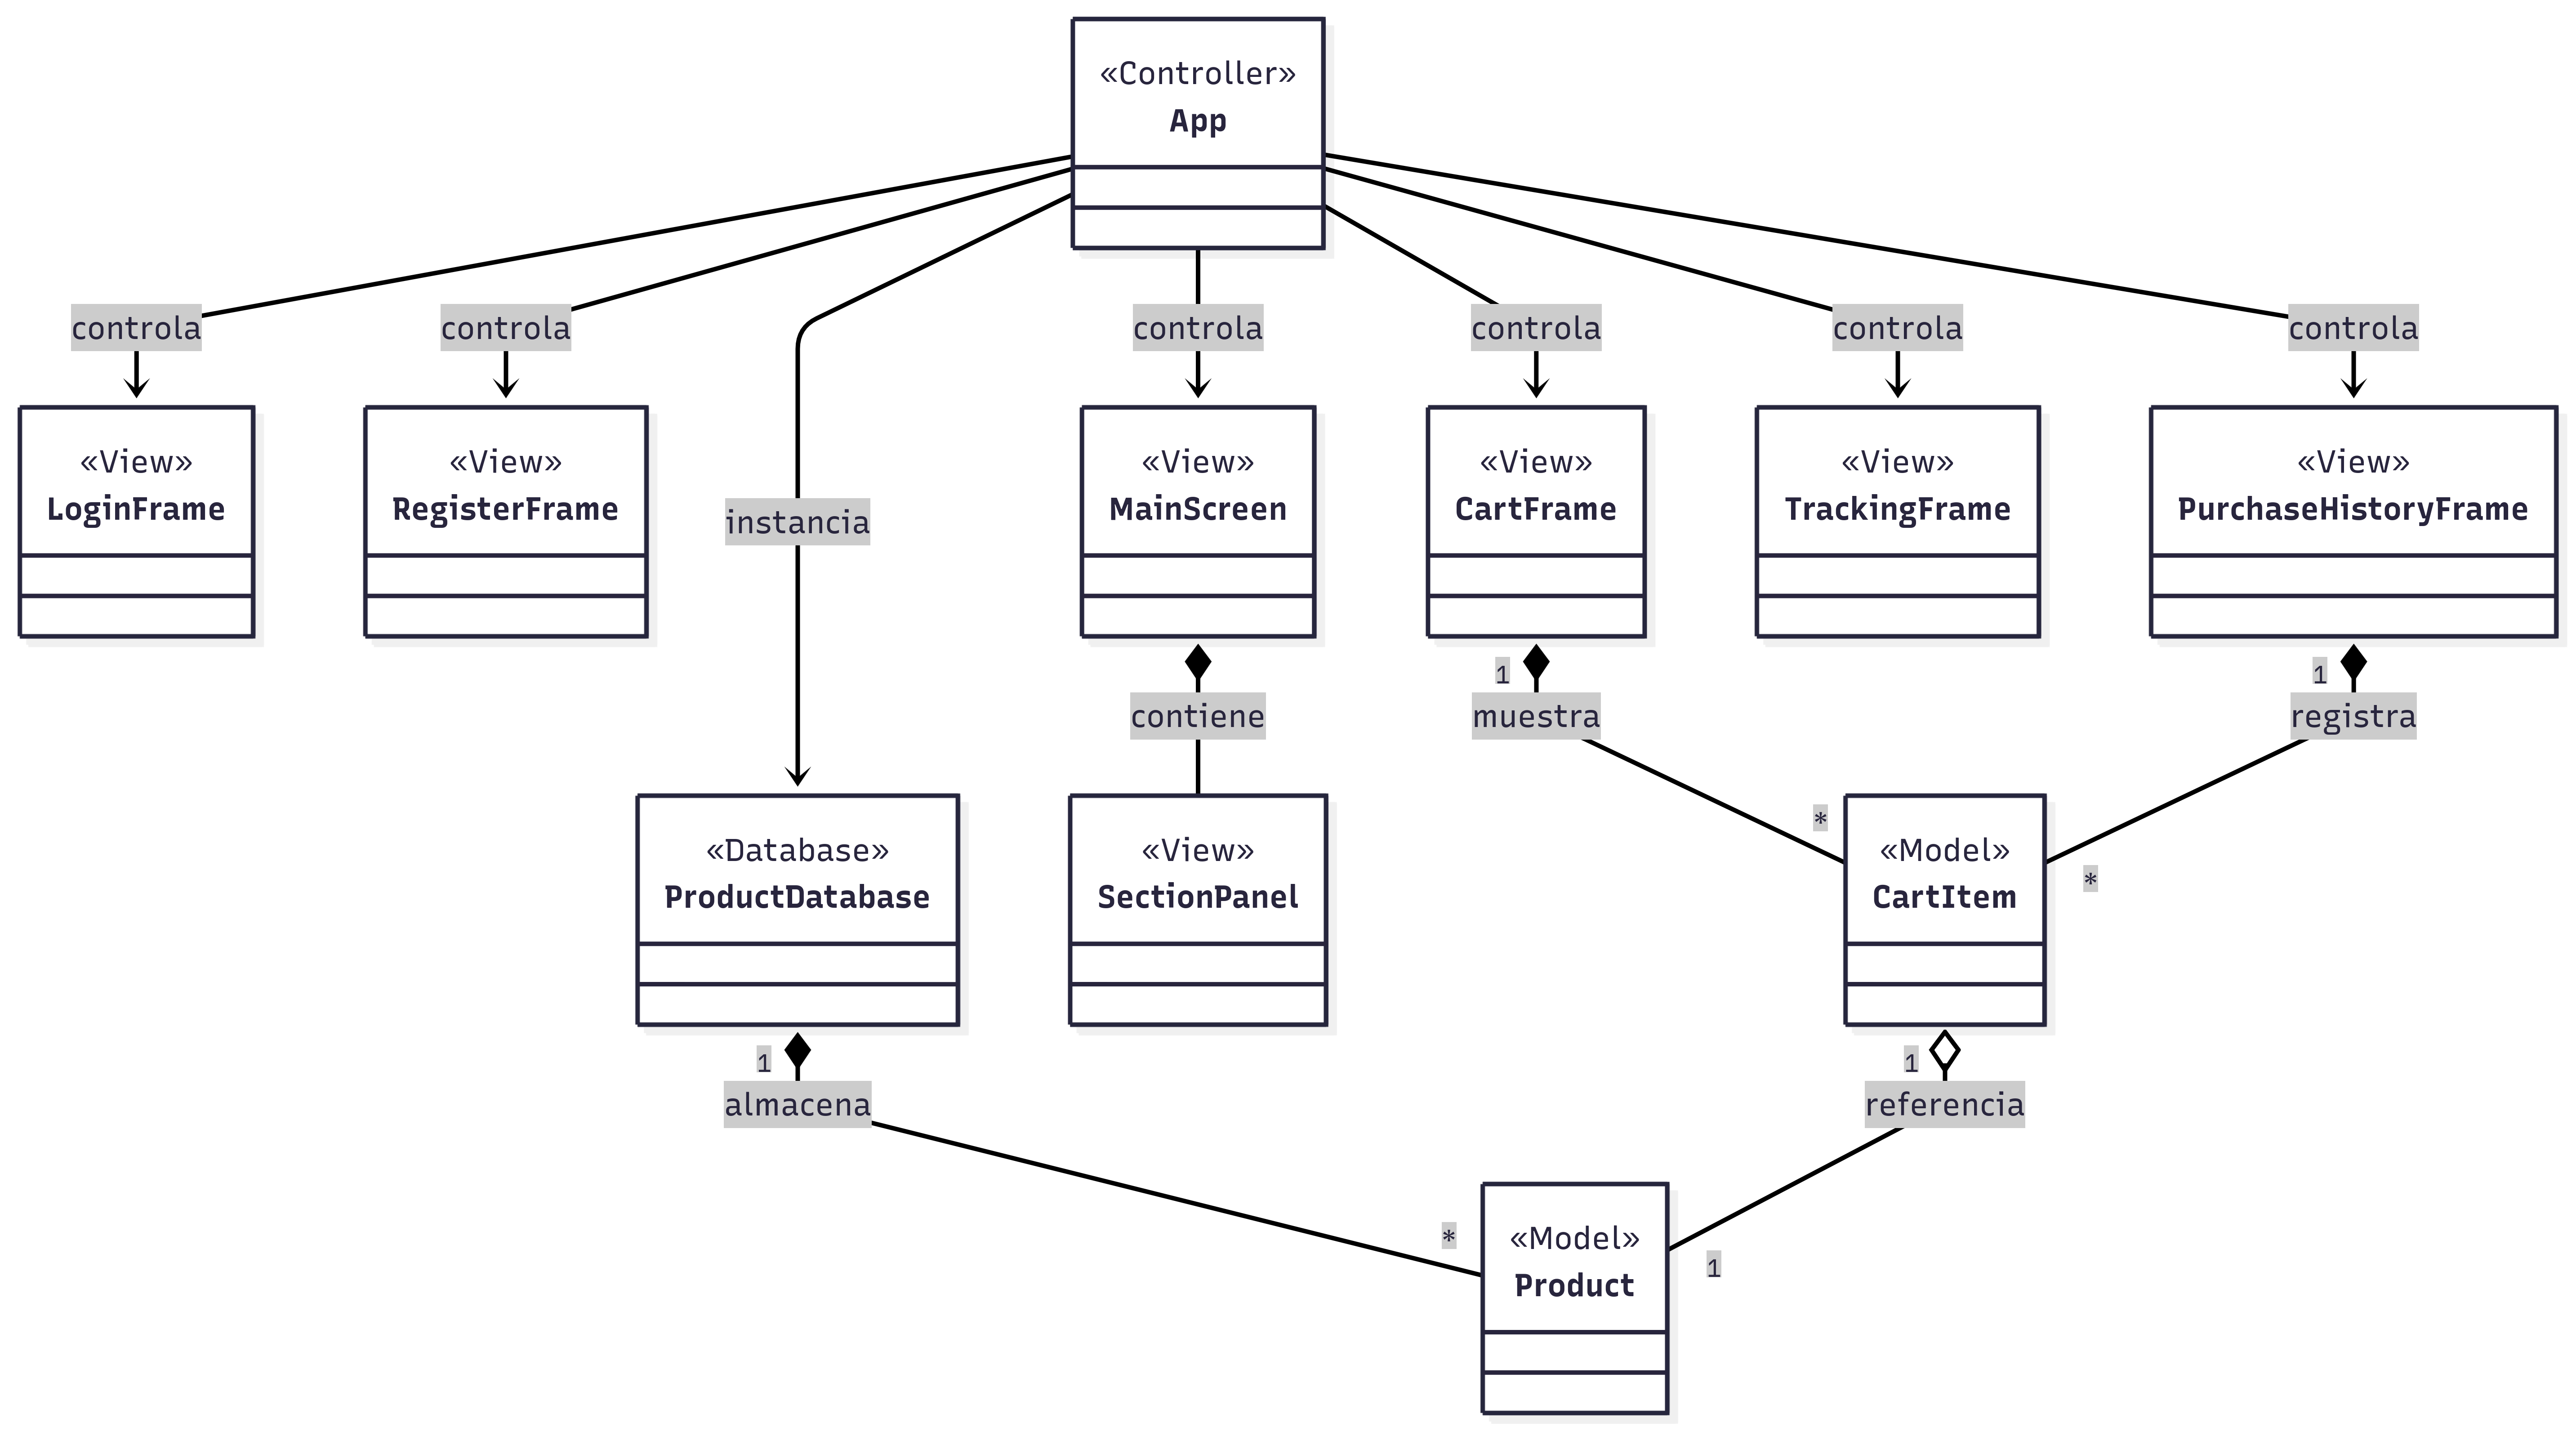
\includegraphics[width=\textwidth]{latex/figure/diagrama_clases.png}
\caption{Diagrama de clases de la aplicación}
\end{figure}

\noindent
\textbf{Descripción:} `App` concentra el estado compartido, la navegación y la autenticación. `LoginFrame` y `RegisterFrame` gestionan el acceso y el alta de usuarios. `MainScreen` muestra la portada con las secciones y productos destacados. `SectionPanel` carga el catálogo de una categoría concreta y `ProductDatabase` centraliza los arrays de productos y la creación de tarjetas visuales. `Product` presenta el detalle de un artículo y permite añadirlo al carrito. `CartFrame` gestiona el carrito activo, `PurchaseHistoryFrame` muestra el historial de compras y `TrackingFrame` representa el seguimiento del último pedido.

\subsubsection*{Diagrama de navegación entre pantallas}
\begin{figure}[H]
\centering
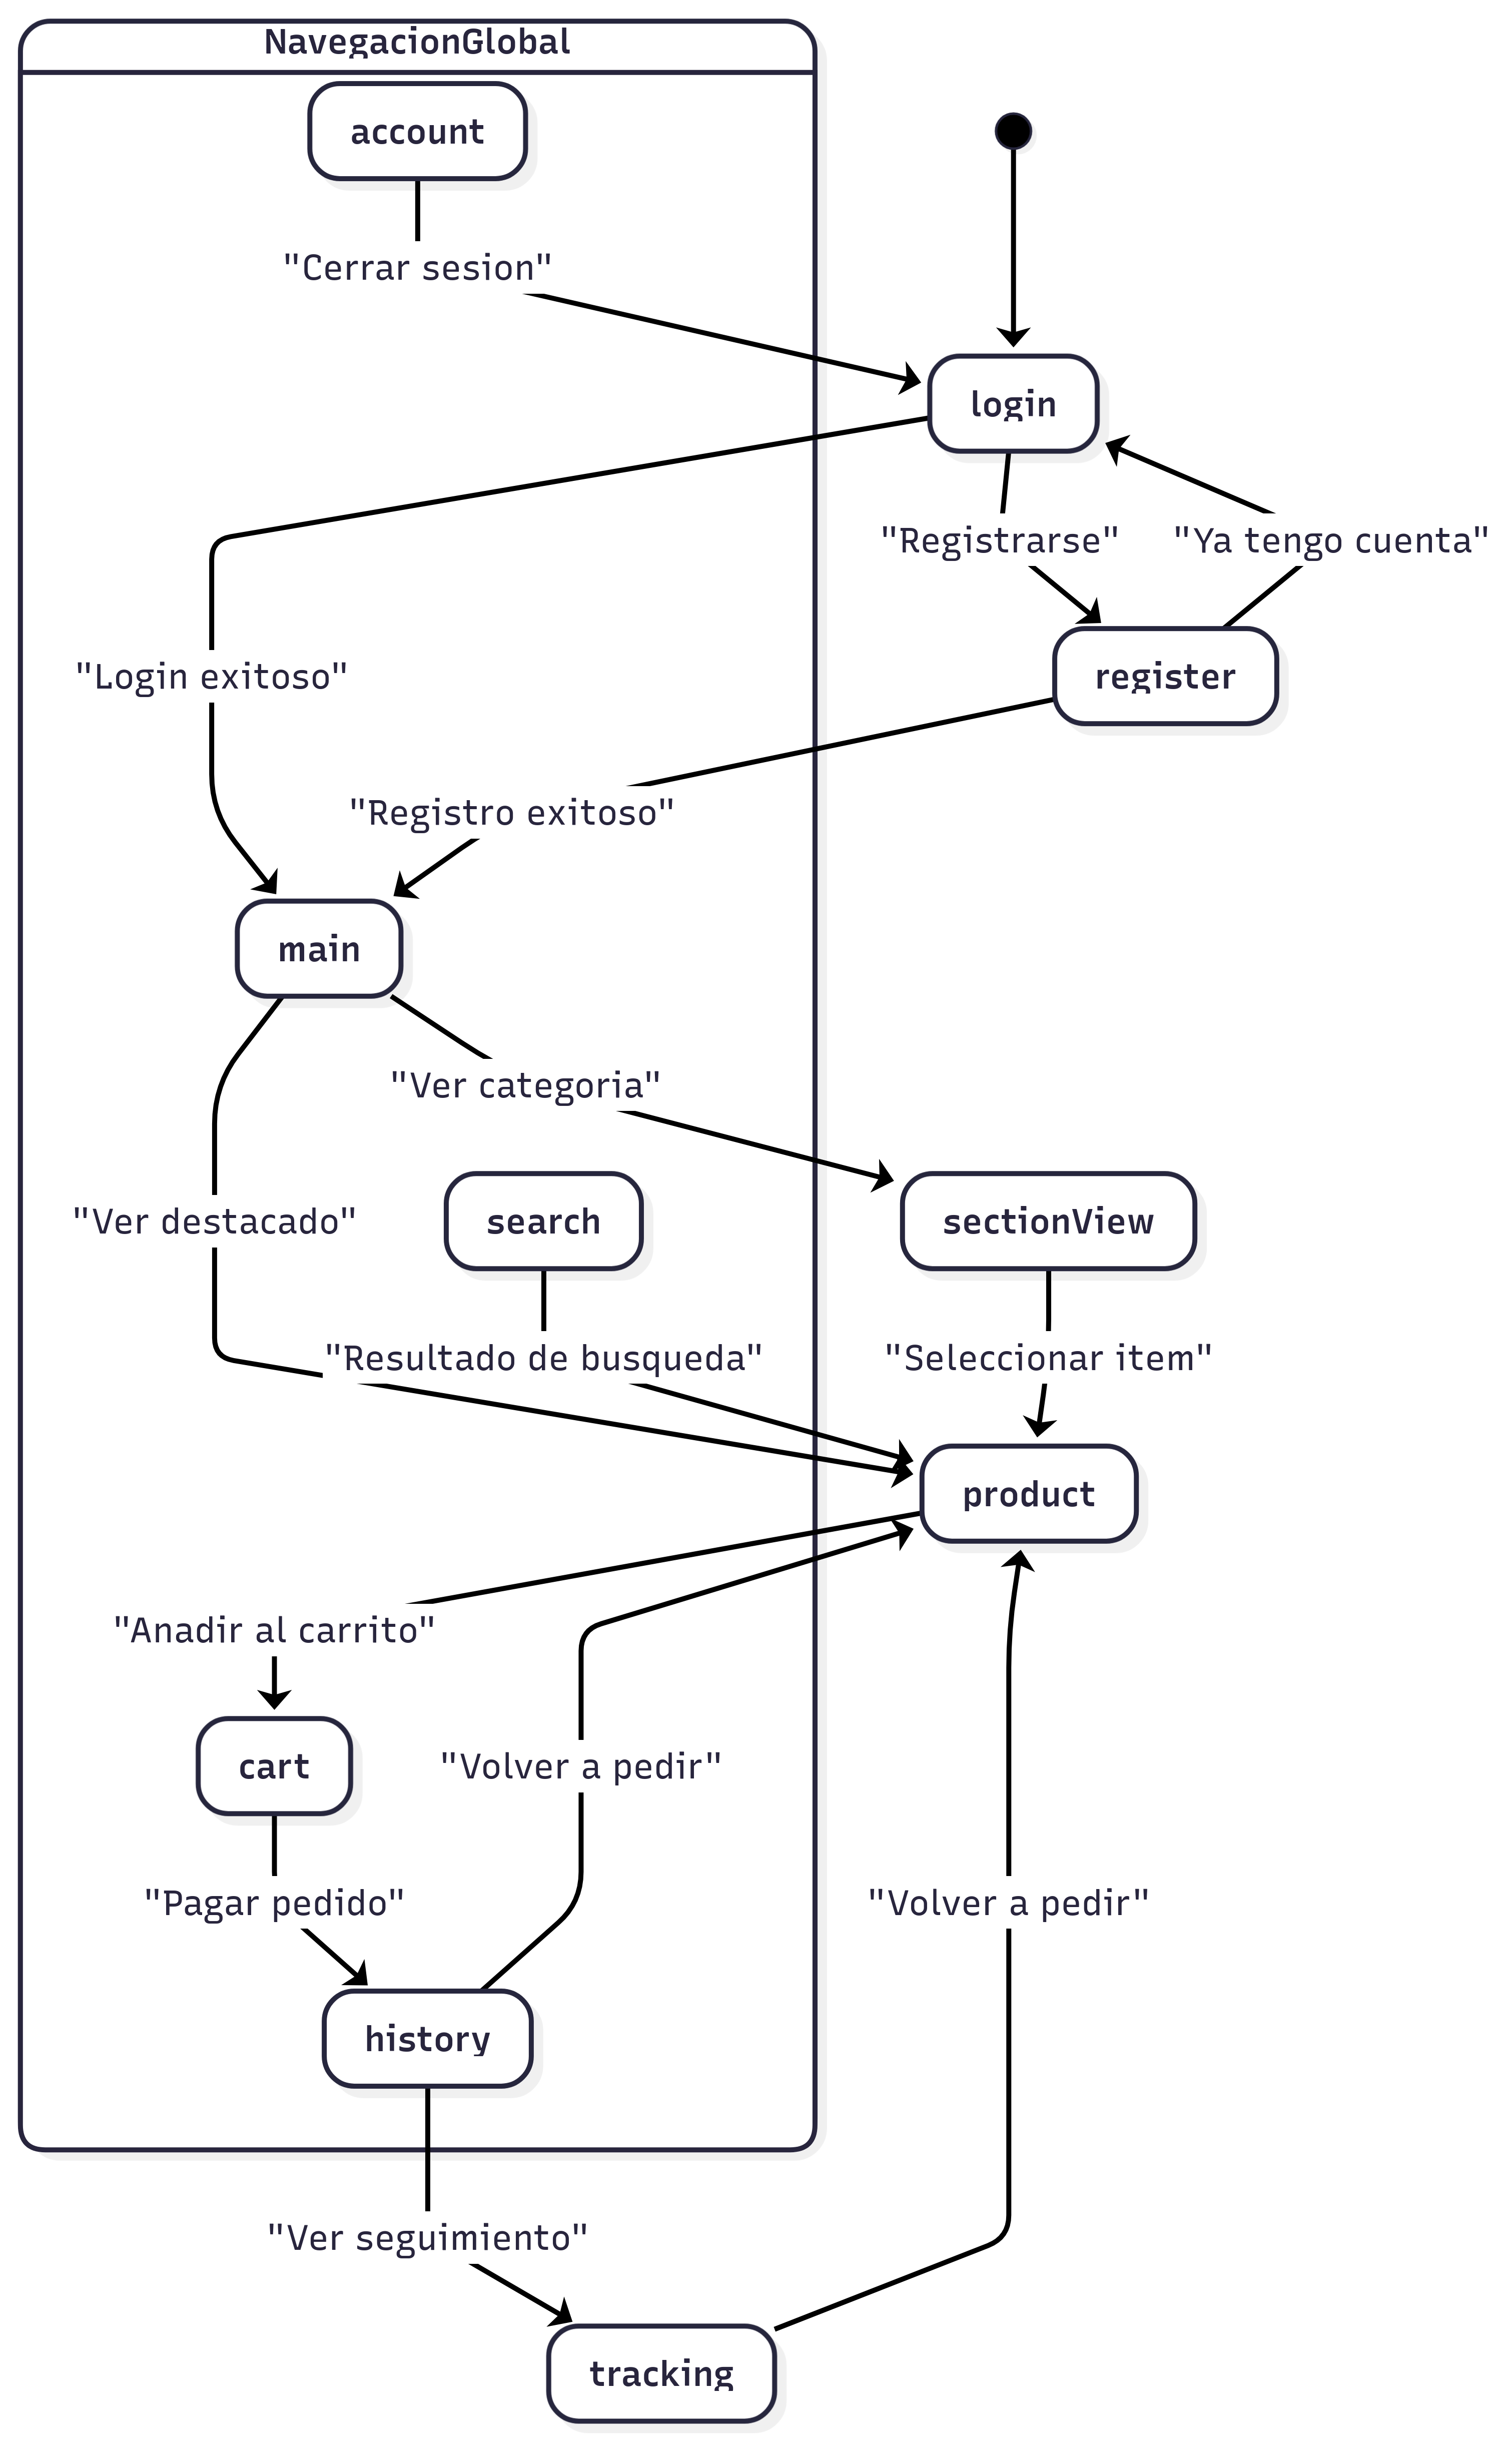
\includegraphics[width=0.7\textwidth]{latex/figure/diagrama_flujo.png}
\caption{Diagrama de navegación entre pantallas}
\end{figure}

\noindent
\textbf{Descripción:} el diagrama extra más útil en este proyecto es el de navegación entre pantallas. Muestra el recorrido login/registro, acceso a la pantalla principal, navegación a catálogo o producto, paso al carrito, consulta del historial y acceso al seguimiento del último pedido.

\subsection{Decisiones de diseño}

\begin{itemize}
	\item \textbf{Consistencia visual:} la interfaz final mantiene una estética identica al prototipo original, aunque pueden existir ajustes de usabilidad o legibilidad.
	\item \textbf{Reutilización de componentes:} se reutilizan paneles redondeados, botones personalizados, la barra de navegación inferior y los mismos estilos tipográficos para mantener coherencia entre pantallas.
	\item \textbf{Separación de responsabilidades:} la interfaz queda en las clases de pantalla, los datos de producto y carrito se encapsulan en \texttt{ProductDatabase} y \texttt{CartItem}, y \texttt{App} centraliza navegación, sesión y estado compartido.
\end{itemize}

\subsection{Internacionalización}

La interfaz está internacionalizada en al menos dos idiomas, tal como exige el enunciado. En esta implementación se han preparado los recursos de texto para permitir el cambio entre idiomas sin modificar la estructura general de la interfaz.

\begin{itemize}
	\item \textbf{Idiomas disponibles:} español e inglés.
	\item \textbf{Archivos de recursos:}\\
	\texttt{src/assets/bundle/Bundle\_es\_ES.properties}\\
	\texttt{src/assets/bundle/Bundle\_en\_GB.properties}
	\item \textbf{Mecanismo de selección:} el selector de idioma en \texttt{LoginFrame}, \texttt{RegisterFrame} y \texttt{Account} cambia el \texttt{Locale} activo y recarga el \texttt{ResourceBundle} sin rehacer la aplicación completa.
	\item \textbf{Textos traducidos:} se traducen etiquetas, títulos, mensajes emergentes, botones de acción y nombres de secciones, de forma que la navegación se mantiene igual en ambos idiomas.
\end{itemize}

\subsection{Aspectos destacados de la implementación}

La interfaz desarrollada no se limita a replicar el aspecto visual del prototipo, sino que integra soluciones estructurales para manejar el estado y la interacción en Swing de forma centralizada. A continuación se detallan los elementos técnicos más relevantes:

\begin{itemize}
	\item \textbf{Gestión dinámica del catálogo:} la vista de productos evita la duplicación de código visual. Las tarjetas de los artículos se generan dinámicamente mediante el método genérico \texttt{createItemCard} en la clase \texttt{ProductDatabase}. Cuando el usuario abre una categoría concreta desde \texttt{MainScreen}, \texttt{SectionPanel} recibe la matriz de datos correspondiente y ensambla la vista al vuelo.
	\item \textbf{Motor de búsqueda unificado:} la barra de búsqueda consolida todas las categorías del inventario en tiempo real utilizando la API de flujos de Java (\texttt{Stream.of().flatMap}). Esto permite filtrar coincidencias en un único array bidimensional, devolviendo los resultados filtrados sin saturar el hilo de eventos de la interfaz.
	\item \textbf{Ciclo de vida del carrito y estado compartido:} los artículos seleccionados se instancian como \texttt{CartItem} y se almacenan en una colección estática dentro de la clase \texttt{App}. La interfaz del carrito no guarda datos, sino que actúa como un visor de esta lista global, calculando el precio total dinámicamente según las cantidades.
	\item \textbf{Persistencia en sesión para historial y seguimiento:} al procesar una compra, el flujo invoca \texttt{App.recordPurchase}. Este método transfiere los elementos del carrito activo al historial general (\texttt{purchaseHistory}), vinculándolos al identificador del usuario autenticado. El panel de seguimiento consulta esta misma estructura para aislar el último pedido realizado.
	\item \textbf{Internacionalización dinámica:} el cambio de idioma no exige reiniciar la aplicación. Al modificar la selección desde la vista de acceso, se actualiza el \texttt{ResourceBundle} global y la aplicación invoca el método \texttt{App.refresh}, el cual recarga las vistas en el \texttt{CardLayout} inyectando las nuevas cadenas de texto sin perder el flujo de navegación.
\end{itemize}

\subsection{Relación con los conceptos teóricos}

\begin{itemize}
	\item \textbf{Visibilidad del estado del sistema y feedback inmediato:} el usuario nunca debe quedar desorientado tras ejecutar una acción. Esto se resuelve mediante el método \texttt{showAppMessage} en la clase \texttt{App}, que despliega un componente flotante efímero (\textit{banner}) controlado por un \texttt{Timer}. Este mecanismo proporciona una confirmación inmediata al añadir un artículo al carrito o procesar un pedido, garantizando que el sistema mantenga siempre informado al usuario de lo que está ocurriendo sin bloquear el hilo principal ni recurrir a diálogos modales disruptivos.
	\item \textbf{Consistencia y estándares:} la consistencia interna se garantiza centralizando la estética y el comportamiento en la clase distribuidora \texttt{App}. La barra de navegación inferior (\texttt{bottomBar}) mantiene un comportamiento predecible gracias a \texttt{updateNavSelection}, que permuta los iconos ordinarios por sus versiones seleccionadas (\textit{Selected.png}), reforzando la noción de ubicación espacial dentro del entorno. Asimismo, el uso sistemático de tipografías específicas (\texttt{Inika-Regular.ttf}) y componentes personalizados como \texttt{RoundedPanel} unifica la experiencia visual en todas las vistas de catálogo.
	\item \textbf{Prevención de errores:} la navegación basada en \texttt{CardLayout} no se gestiona de forma libre o descontrolada, sino mediante una pila acotada de historial (\texttt{navigationHistory} implementada con un \texttt{ArrayDeque}). Al limitar el rastro a un máximo de cinco pantallas (\texttt{MAX\_NAV\_HISTORY = 5}), se evita que el usuario quede atrapado en bucles infinitos al usar el botón de retroceso. Del mismo modo, el método \texttt{isTransientScreen} aísla los estados de inicio de sesión y registro, impidiendo un retroceso ilegal a pantallas de autenticación una vez que la sesión está activa y el estado global ha cambiado.
	\item \textbf{Flexibilidad y eficiencia de uso:} la interfaz se adapta dinámicamente al contexto del usuario. En lugar de construir paneles estáticos para cada categoría de productos, la arquitectura utiliza \texttt{ProductDatabase.createItemCard} para generar elementos de interfaz al vuelo basándose en las matrices de datos solicitadas por \texttt{SectionPanel}. Esto optimiza el rendimiento de la aplicación en memoria y reduce la carga cognitiva del usuario al presentar la información estructurada bajo un mismo patrón de interacción, independientemente de la sección consultada.
\end{itemize}


\subsection{Cambios respecto al prototipo}
A continuación se detalla todos los cambios respecto al prototipo de la primera entrega:
\begin{itemize}
    \item \textbf{Uso de pestañas de dialogos:} Se ha decidido el uso de dialogos con un temporizador para avisar al usuario de distintas cosas como que tiene que rellenar algun campo o se ha añadido un elemento al carrito.
        \begin{center}
        
\includegraphics[width=0.5\linewidth]{latex/figure/Dialogo.png}
        \captionof{figure}{Ejemplo Dialogo}
        \end{center}
    \item \textbf{Desplegable de idioma en el login:} Se ha decidido poner el desplegable de idioma del apartado de \textbf{Cuenta} para que el usuario no tenga que ir por todo el flujo de la aplicación para cambiar de idioma y pueda hacerlo desde la primera pantalla.
        \begin{center}
        
\includegraphics[width=0.3\linewidth]{latex/figure/Idioma.png}
        \captionof{figure}{Idioma Login}
        \end{center}
    \item \textbf{Modal de dirección:} Se ha introducido un modal a la hora de pagar para tener el campo dirección del usuario.
        \begin{center}
        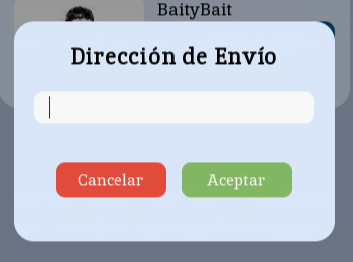
\includegraphics[width=0.5\linewidth]{latex/figure/direccion.png}
        \captionof{figure}{Modal dirección}
        \end{center}
    \item \textbf{Flechita para retroceder:} Se ha añadido una flechita hacia atrás que lleva a la pantalla anterior, esto mejora el flujo de trabajo y la navegación por la aplicación.
        \begin{center}
        
\includegraphics[width=0.2\linewidth]{latex/figure/back.png}
        \captionof{figure}{Flechita atrás}
        \end{center}
\end{itemize}

\section{Tutorial o breve manual de usuario}

\subsection{Requisitos previos}

\begin{itemize}
	\item Java 17 o superior.
	\item Un entorno con \texttt{javac} y \texttt{java} disponibles.
	\item No se requieren dependencias externas adicionales.
\end{itemize}

\subsection{Compilación}
Se incluye un script de construcción que compila las clases, empaqueta los recursos y genera un fichero JAR ejecutable.

\begin{enumerate}
	\item Abrir una terminal en la raíz del proyecto.
	\item Hacer ejecutable el script de construcción: \texttt{chmod +x build.sh}.
	\item Ejecutar el script para compilar y empaquetar: \texttt{./build.sh}.
\end{enumerate}

\begin{verbatim}
./build.sh
\end{verbatim}

\subsection{Ejecución}

Para ejecutar la aplicación desde el JAR generado:

\begin{verbatim}
java -jar uco-si-final.jar
\end{verbatim}

Si necesita ejecutar sin usar el JAR, puede compilar y ejecutar en el classpath:
\begin{verbatim}
javac -d bin src/*.java
java -cp bin App
\end{verbatim}

\subsection{Uso de la aplicación}

El recorrido del usuario se ha estructurado de manera secuencial para que resulte intuitivo, imitando la dinámica de una tienda virtual tradicional. A continuación, se detalla el flujo principal paso a paso:

\begin{enumerate}
	\item \textbf{Autenticación y configuración:} Al arrancar el programa, la vista inicial solicita iniciar sesión con una cuenta existente (correo y contraseña) o crear una cuenta nueva desde el formulario de registro. Por defecto, la aplicación incluye una cuenta de prueba con\newline el correo \textbf{el\_pescador@gmail.com} y la contraseña \textbf{MeGustanLosPeces123}. Antes de acceder, un selector en la esquina superior permite cambiar el idioma entre español e inglés directamente desde la pantalla de acceso o registro.
	\item \textbf{Navegación principal:} Una vez dentro de la sesión, el usuario dispone de una barra inferior persistente. Esta herramienta sirve para navegar de forma rápida hacia las áreas de inicio, búsqueda, carrito, historial o cuenta, independientemente de la vista actual.
	\item \textbf{Exploración de productos:} En la pantalla de inicio, se puede entrar en una sección específica (como anzuelos, cañas o cebos) para explorar esa categoría. Al pulsar sobre la tarjeta de un producto, la interfaz muestra su ficha con descripción y precio, permitiendo añadirlo al carrito desde allí. Como alternativa, la sección de búsqueda filtra coincidencias de texto en todo el catálogo.
	\item \textbf{Gestión y confirmación de compra:} La vista del carrito permite revisar los artículos seleccionados y ajustar cantidades con botones interactivos. Para completar la compra, el botón "Pagar" despliega un panel modal que exige introducir una dirección de envío. Al confirmar los datos, el sistema finaliza el pedido, vacía el carrito actual y guarda la información en el historial para su seguimiento posterior.
\end{enumerate}

\newpage
\subsection{Manual de usuario}

Se incluyen a continuación las capturas de las pantallas principales. Ademas de una explicación de hacia donde lleva cada boton.
\begin{figure}[H]
\centering
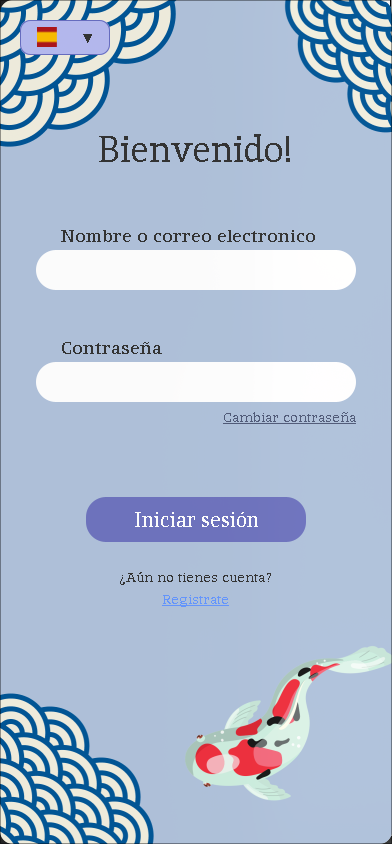
\includegraphics[width=0.5\textwidth]{latex/interface/login.png}
\caption{Pantalla de inicio de sesión}
\end{figure}

\noindent
\textbf{Descripción:} Inicio de sesión, para poder entrar hay que rellenar correctamente los campos y darle al botón de \texttt{Iniciar Sesión}. Además tenemos la opción de darle a \texttt{Registrate} que nos enviará a la pantalla de registro, o \texttt{Cambiar Contraseña} el cual simulará enviar un correo al correo que este en el campo de correo en ese momento. Finalmente con el desplegable de la esquina se podrá cambiar de idiomas.

\begin{figure}[H]
\centering
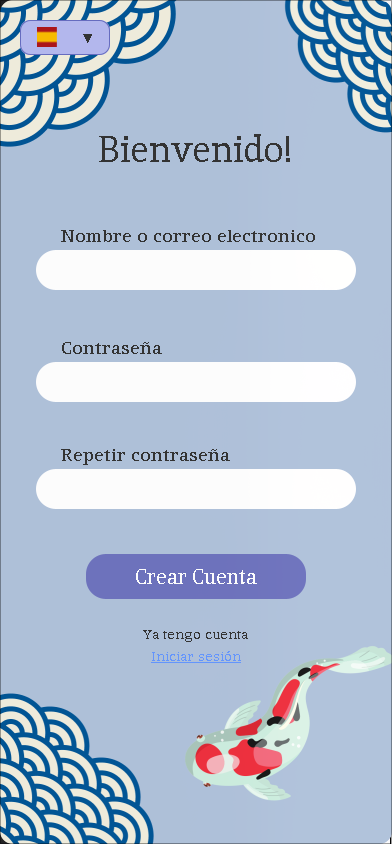
\includegraphics[width=0.5\textwidth]{latex/interface/register.png}
\caption{Pantalla de registro}
\end{figure}

\noindent
\textbf{Descripción:} Formulario para crear una cuenta nueva con los mismos controles de idioma y acceso que la pantalla de inicio. Funciona de manera similar al anterior añadiendo el campo de \texttt{Repetir Contraseña} y \texttt{Iniciar Sesión}, que volverá a la pestaña anterior.

\begin{figure}[H]
\centering
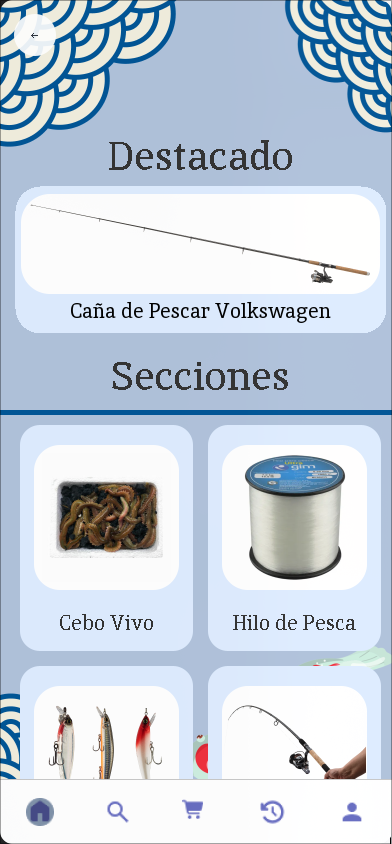
\includegraphics[width=0.5\textwidth]{latex/interface/mainScreen.png}
\caption{Pantalla principal}
\end{figure}

\noindent
\textbf{Descripción:} Vista de entrada a la aplicación con acceso a las secciones, productos destacados y navegación inferior. Si clickas en los productos destacados nos llevará a la página específica de cada uno. Sin Embargo si clickas en una sección nos listará todos los productos que correspondan a esa sección.




\begin{figure}[H]
\centering
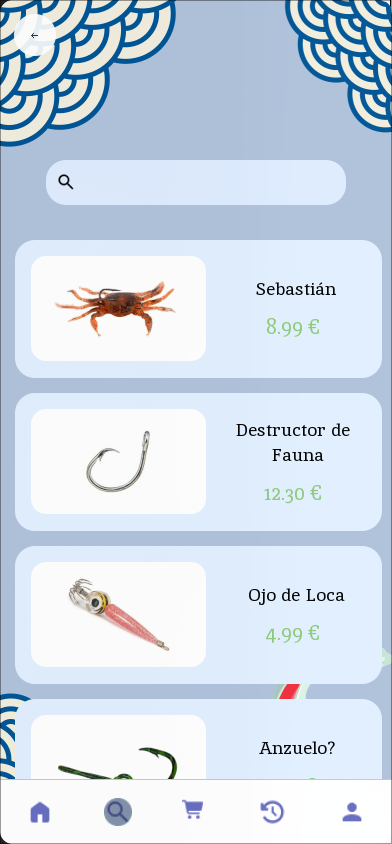
\includegraphics[width=0.5\textwidth]{latex/interface/search.png}
\caption{Pantalla de búsqueda o catálogo}
\end{figure}

\noindent
\textbf{Descripción:} Catálogo filtrable donde el usuario localiza productos por nombre antes de abrir su ficha. Si quiere ver más detalles o comprar el usuario puede clickar en un producto y se verá la página detallada del producto.

\begin{figure}[H]
\centering
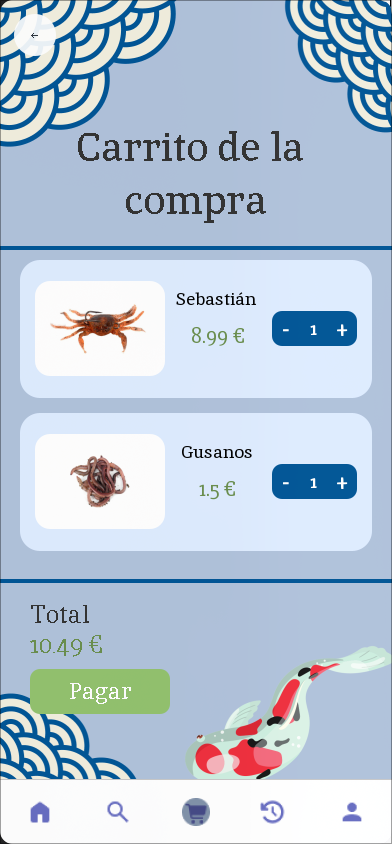
\includegraphics[width=0.5\textwidth]{latex/interface/shoppingCart.png}
\caption{Pantalla del carrito}
\end{figure}

\noindent
\textbf{Descripción:} Resumen de los productos añadidos, con ajuste de cantidades, cálculo del total y acceso al proceso de compra. Si le damos a pagar, nos saldŕa un modal preguntando por nuestra dirección de envio antes de darle a aceptar.

\begin{figure}[H]
\centering
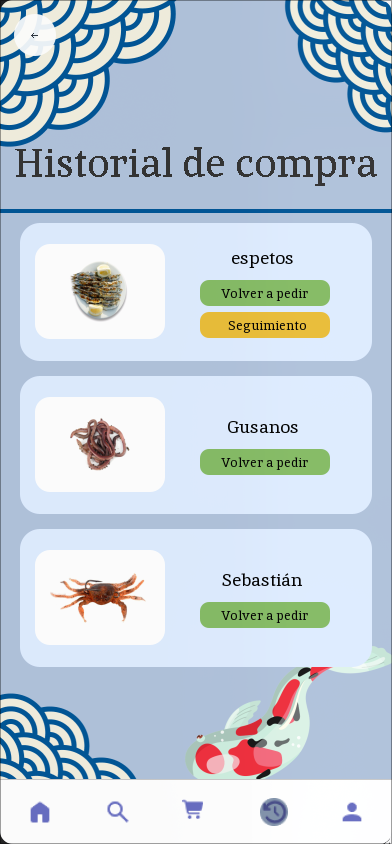
\includegraphics[width=0.5\textwidth]{latex/interface/history.png}
\caption{Pantalla de historial de compras}
\end{figure}

\noindent
\textbf{Descripción:} Listado de pedidos realizados por el usuario con los elementos de cada compra y su información básica. Para esta simulación los productos de la última compra son los que no se han entregado, por tanto a parte de la opción de \texttt{Volver a comprar} que estará en todos los productos y llevará a la página de detalles del producto. Y la de seguimiento tendrá un seguimiento del producto hasta llegar al destino.

\begin{figure}[H]
\centering
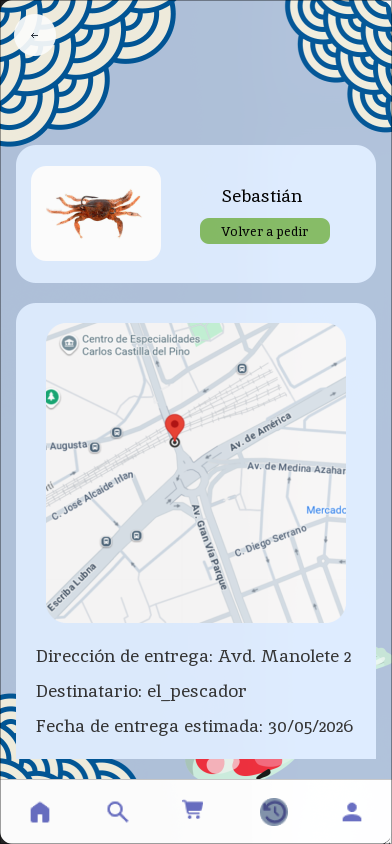
\includegraphics[width=0.5\textwidth]{latex/interface/tracking.png}
\caption{Pantalla de seguimiento}
\end{figure}

\noindent
\textbf{Descripción:} Vista de seguimiento del último pedido para consultar el estado de la compra y sus detalles. Similar a la anterior, el botón de \texttt{Volver a comprar} lleva a la página del producto.

\begin{figure}[H]
\centering
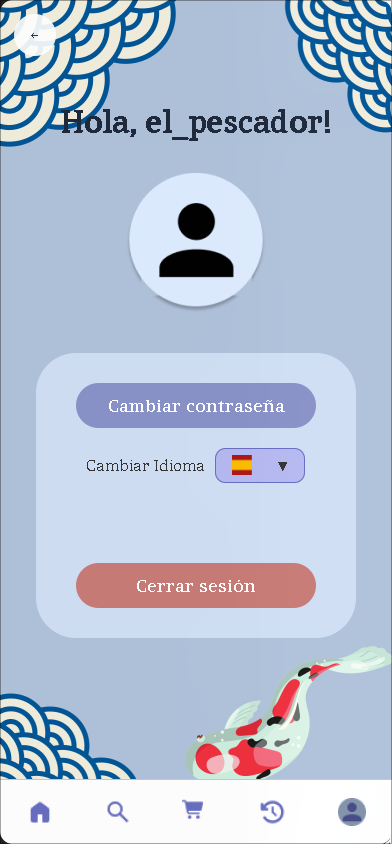
\includegraphics[width=0.5\textwidth]{latex/interface/account.png}
\caption{Pantalla de cuenta}
\end{figure}

\noindent
\textbf{Descripción:} Panel de cuenta del usuario con información personal y opciones asociadas a su sesión. Tenemos la opción de \texttt{Cerrar Sesión} que nos llevará al login de nuevo, el cambio de contraseña que es similar al del login, y el desplegable del idioma.

\section{Conclusiones}

En esta sección se deben resumir los resultados obtenidos, las dificultades encontradas y una valoración final de la solución desarrollada.

\subsection*{Resultados}
Se ha cumplido el objetivo principal: la aplicación cuenta con una interfaz funcional, navegación entre pantallas, catálogo de productos, búsqueda, carrito, historial, seguimiento y cambio de idioma. La principal limitación es que varias partes siguen apoyándose en datos de prueba y quedan capturas o diagramas por sustituir en la memoria.

\subsection*{Dificultades y mejoras futuras}
\begin{itemize}
	\item La adaptación del prototipo a Swing obligó a ajustar tamaños y contenedores; se resolvió unificando paneles redondeados y layouts reutilizables.
	\item La internacionalización exigió centralizar textos en \texttt{ResourceBundle}; con ello se evitó duplicar la interfaz para cada idioma.
	\item Como mejora futura, conviene persistir usuarios y compras en disco o base de datos.
	\item También sería útil completar la compra con validaciones más realistas y sustituir todos los recursos provisionales.
\end{itemize}

\subsection*{Valoración final}
En conclusión, el diseño de un prototipo ha demostrado ser una herramienta fundamental para la viabilidad y calidad del proyecto (a pesar de que haya cosas que no podemos cumplir). Disponer de una maqueta visual interactiva ha permitido evaluar de forma tangible el flujo de la aplicación e identificar fallos de usabilidad.
\appendix
\section{Anexos}

\subsection{Referencias de recursos}
\begin{itemize}
	\item Recursos gráficos incluidos en \texttt{src/assets/}.
	\item Documentación de Java Swing y de \texttt{ResourceBundle}.
	\item https://gemini.google.com/app
\end{itemize}

\end{document}
